\chapter{Meet the Billionaire Who Created LinkedIn (Then Sold It for \$26B)}

This chapter has almost no blackboard mathematics in the ordinary sense, but it is mathematical all the same. The interview turns on filters, thresholds, repeated play, compounding, and the logic of network growth. We are shown the outcome first: a \$26 billion exit, a business that later produced roughly \$16 billion in annual revenue, a founder whom more than two-thirds of his smart friends expected to fail, and a venture world in which hundreds of annual pitches narrow to almost no investments. Only after that spectacle do we return to the real subject: what kind of reasoning allows a person to commit early, survive failure, and build value that is not yet visible.

\section{Cold Open: Outcome, Doubt, and Filter Math}

The lecture opens in the style of a teaser reel. Before any doctrine is stated, we are given a cluster of scale markers. They function as numerical stakes, not yet as explanation. In that opening sequence, the interview places side by side LinkedIn, Microsoft, the PayPal network, venture-capital selectivity, the Airbnb anecdote, and the emergency question of how one might try to make a billion dollars in a year.

\begin{align}
V_{\mathrm{LI,sale}} &= \$26\,\mathrm{B}, &
R_{\mathrm{LI,last}} &\approx \$16\,\mathrm{B/yr}, \\
V_{\mathrm{PayPal,sale}} &\approx \$1.5\,\mathrm{B}, &
d &> \frac{2}{3}, \\
N_{\mathrm{deals}} &\in [600,800], &
N_{\mathrm{yes}} &\in [0,2].
\end{align}

Here \(d\) is the fraction of Hoffman's smart friends who thought LinkedIn would fail. The numbers are worth keeping separate. The sale price of LinkedIn is not the same thing as personal annual income, and the later annual revenue of LinkedIn is not the same thing as the sale price. The interview itself slides quickly between these scales because it is staging magnitude. Our notes should distinguish them.

The venture-capital numbers already suggest the first mathematical lesson. A founder is not entering a neutral marketplace of ideas; he is entering an extreme filter.

\paragraph{Worked filter.}
If we take the optimistic end of Hoffman's own counts, then the implied acceptance rate is bounded above by
\begin{equation}
p_{\mathrm{yes}}=\frac{N_{\mathrm{yes}}}{N_{\mathrm{deals}}}\lesssim \frac{2}{600}\approx 3.3\times 10^{-3}.
\end{equation}
That is less than one third of one percent. If we take the pessimistic end, the rate is \(0\). The point is not the exact fraction; the point is that ordinary plausibility is not enough. A founder must have a view of the world that survives brutal compression.

\begin{figure}
\begin{center}
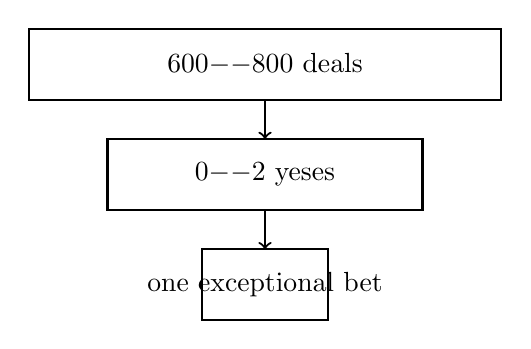
\begin{tikzpicture}
\draw[thick] (0,0) rectangle (6,0.9);
\draw[thick] (1.0,-1.4) rectangle (5.0,-0.5);
\draw[thick] (2.2,-2.8) rectangle (3.8,-1.9);
\draw[->,thick] (3,0) -- (3,-0.5);
\draw[->,thick] (3,-1.4) -- (3,-1.9);
\node at (3,0.45) {$600\text{--}800$ deals};
\node at (3,-0.95) {$0\text{--}2$ yeses};
\node at (3,-2.35) {one exceptional bet};
\end{tikzpicture}

{\small A transcript-derived schematic of the venture filter described in the interview.}
\end{center}
\end{figure}

The lecture does not linger here. It immediately adds two more signals. First, when Hoffman met the Airbnb founders, he says he knew within two minutes that he wanted to invest. Second, when the host asks for a one-year path to a billion dollars, Hoffman later refuses the frame and moves us toward a ten-year game. So even in the cold open, the deep structure is already visible: selection, surprise, and horizon.

\section{Burn the Boats Early, but Preserve the Right to Play Again}

After the travel setup and a brief editorial jump in the transcript, the interview resets into chronology. We are taken back to ``the early days'' of LinkedIn and asked for the moment when Hoffman knew he would go all in. His answer is exact and somewhat contrary to popular entrepreneurial mythology. We do not wait for confidence and then commit. We commit before confidence is available.

The lecture's first principle can be written as a simple inequality. A worthwhile entrepreneurial risk is not a risk with no downside. It is a risk with enormous upside and a downside that does not destroy the ability to re-enter the game:
\begin{equation}
U_{\mathrm{win}} \gg L_{\mathrm{fail}}, \qquad L_{\mathrm{fail}} < L_{\mathrm{ruin}}.
\end{equation}
The first inequality captures asymmetry: if it works, it works big. The second captures survivability: if it fails, we are still alive in the strategic sense. We may play again.

\begin{definition}
A repeatable entrepreneurial risk is a risk for which the upside is disproportionately large, the failure cost is real but tolerable, and the outcome does not destroy future optionality.
\end{definition}

What matters here is that ``burn the boats'' does not mean theatrical recklessness. It means that hesitation cannot be the governing principle in a domain where advantage comes from acting before social consensus has formed.

\subsection{Question \& Answer}

\paragraph{Question.}
Why commit before we feel certain?

\paragraph{Answer.}
Because certainty arrives too late. If a path is already obviously safe, then the edge has probably disappeared. The lecture's answer is not that fear vanishes; Hoffman explicitly says everyone is a little afraid of failure. The answer is that we structure the wager so that fear is not terminal. We accept that the move may fail, but we insist that failure not become ruin. In that sense the lecture replaces the romance of courage with the engineering of replay.

This is why Hoffman says he learned from earlier ventures and from PayPal. The founder's problem is not to eliminate uncertainty. The founder's problem is to enter uncertainty on terms that preserve another move.

\section{Choosing the Right Game and the Right Geography}

The conversation then asks a sharper question: where did the confidence come from? Hoffman's answer is not simply self-belief. He says he knew what strategic game he was playing, and he knew where that game could be played best. The lecture now moves from personal commitment to strategic placement.

A compact way to write this is
\begin{equation}
g(\mathrm{Silicon\ Valley})=\mathrm{software}, \qquad
g(\mathrm{New\ York})=\mathrm{finance}, \qquad
g(\mathrm{Los\ Angeles})=\mathrm{media}.
\end{equation}
This is not a law of nature. It is a strategic map. The point is that domains cluster, and a founder's confidence may come from being in the place where the relevant institutions, talent, and habits already exist.

This also clarifies the earlier point about repeated play. If we know which game we are playing, and if we know that the arena supports multiple attempts, then failure in one move does not force exit from the entire field. The ability to play again is not only personal. It is ecological. Silicon Valley, in Hoffman's telling, is not just a place to win; it is a place to attempt, fail, learn, and attempt again inside the same general strategic universe.

From here the lecture turns naturally to the harder question. Even if software in Silicon Valley was the right game, why was LinkedIn itself not a bad bet? Why did so many smart observers think it would fail?

\section{The Network Bootstrap Problem at LinkedIn}

Now we reach the cleanest conceptual obstacle in the interview. Hoffman says that in 2003 many people in Silicon Valley thought the consumer internet was over. Amazon, Google, and PayPal were already visible, but the next wave of consumer social products did not yet have legitimacy. LinkedIn, in particular, sounded to skeptics like a vague professional variant of an already dubious category.

The objection he reports is precise. A network has no value at the beginning. The first person in gets no value. The next few people may already know one another, so again there seems to be no value. Then why should the thing grow at all?

A cautious reconstruction of the argument is
\begin{equation}
V_{\mathrm{net}}(n)\approx 0 \qquad \text{for very small } n,
\end{equation}
together with the claim that beyond some threshold \(n_\ast\), the marginal value becomes positive in a meaningful way:
\begin{equation}
V'_{\mathrm{net}}(n)>0 \qquad \text{once the network is thick enough to create real reach and matching.}
\end{equation}
The transcript does not provide a formula for \(V_{\mathrm{net}}(n)\), so we should not invent one. What it does provide is the qualitative shape: a flat and discouraging early region, followed by a regime in which accumulated participation begins to matter.

\begin{figure}
\begin{center}
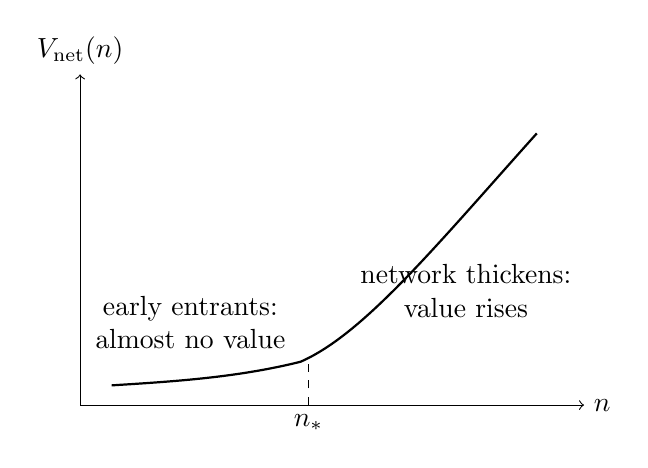
\begin{tikzpicture}[scale=1.0]
\draw[->] (0,0) -- (6.4,0) node[right] {$n$};
\draw[->] (0,0) -- (0,4.2) node[above] {$V_{\mathrm{net}}(n)$};
\draw[thick] (0.4,0.25) .. controls (1.2,0.30) and (2.0,0.35) .. (2.8,0.55)
             .. controls (3.6,0.90) and (4.5,2.00) .. (5.8,3.45);
\draw[dashed] (2.9,0) -- (2.9,0.62);
\node[below] at (2.9,0) {$n_\ast$};
\node[align=center] at (1.4,1.05) {early entrants:\\almost no value};
\node[align=center] at (4.9,1.45) {network thickens:\\value rises};
\end{tikzpicture}

{\small A transcript-derived sketch of the network bootstrap problem that Hoffman says many skeptics missed.}
\end{center}
\end{figure}

\subsection{Question \& Answer}

\paragraph{Question.}
How can a network with no initial value still become valuable?

\paragraph{Answer.}
The lecture's answer is not that the first users were secretly receiving large value. It is that the founder only needs a path by which participation continues long enough for the value curve to bend upward. If professional identity, invitations, or the promise of future reach can keep pushing \(n\) upward, then the system may cross a threshold where matching, search, reputation, and access begin to emerge from the aggregate.

\paragraph{A small derivation.}
We can summarize the bootstrap logic in four steps:
\begin{enumerate}
\item For \(n\) very small, \(V_{\mathrm{net}}(n)\) is nearly zero.
\item This produces the obvious criticism: no immediate value, therefore no growth.
\item The founder's contrarian thesis \(\theta\) is that there exists a credible path from small \(n\) to threshold \(n_\ast\).
\item Once \(n\geq n_\ast\), each additional participant raises the usefulness of the whole network, so growth and value begin to reinforce each other.
\end{enumerate}

This is exactly where the interview's recurring question appears in its sharpest form: what did Hoffman know that others did not know? His answer is not mystical. It is structural. He believed the network could be made to grow before its value was obvious to its early users.

\section{From Civil Servants to Product Creation}

After the network puzzle, the lecture broadens briefly into biography. Hoffman says he did not come from a family of entrepreneurs but from a family of civil servants. His grandfather apparently saw industrial life with some suspicion. This matters because it makes the entrepreneurial turn less like inheritance and more like strategic self-construction.

The turning point, as Hoffman tells it, comes through Stanford, artificial intelligence, and then a clearer desire: not simply to work at companies, but to create new products. Apple and Fujitsu appear in this part of the story, not as final destinations, but as stations on the way to product-making. The lecture is careful here. The founder is not born fully armed. He becomes the kind of person who prefers building new things over occupying existing roles.

This brief section also prepares a later transition. When the interview returns to money, exits, and relationships, it is no longer enough to know that LinkedIn became large. We now need to understand how a builder becomes legible to other powerful builders.

\section{Credibility, Networking, and Real Connection}

When the interview returns after a long promotional interruption, the question is no longer how to start a company but how to build relationships with serious operators. Hoffman's answer is clear and beautifully non-theatrical. The first move in networking is not to ask. It is to give.

A useful schematic is
\begin{equation}
C_{t+1}=C_t+\Delta C(U_t),
\end{equation}
where \(C_t\) denotes relationship capital at time \(t\), and \(U_t\) denotes the usefulness of what we offer. The lecture's claim is not that all useful gestures are rewarded. It is that genuine usefulness is the proper state variable. Asking first, before offering anything, is usually a bad update rule.

We may sharpen the contrast by saying: when the encounter is merely extractive, the increment is weak or negative; when it is genuinely helpful, the relation begins to accumulate.
\begin{equation}
U_t>0 \Longrightarrow \Delta C(U_t)>0,
\qquad
U_t=0 \text{ with ask-first behavior } \Longrightarrow \Delta C(U_t)\leq 0.
\end{equation}

The examples in the transcript are concrete. Satya Nadella calls Hoffman because Hoffman can explain Silicon Valley. Bill Gates is not approached through flattery but through information: here is something happening in modern technology, perhaps in AI, that you may not yet have seen. In both cases the mechanism is the same. Access follows usefulness.

\subsection{Question \& Answer}

\paragraph{Question.}
How do we build relationships with A players before we have much credibility?

\paragraph{Answer.}
Not by pretending to already possess their status, and not by handing over a business card as if the exchange itself created substance. We build the relation by bringing an observation, an introduction, a synthesis, or a pattern that is actually useful. The lecture insists that real networking is not symbolic contact; it is mutual help.

Hoffman then identifies three recurring qualities among elite operators:
\begin{itemize}
\item curiosity, or the intense desire to learn;
\item grit, or the insistence on making the thing work;
\item contrarian understanding, or a live hypothesis about what others do not yet understand.
\end{itemize}
The third of these returns us to the earlier theme. Networking is not separable from thought. To be useful to strong people, one must have seen something worth bringing to them.

This is also why Hoffman dismisses much of ordinary networking as empty ritual. ``Hi, I'm Reid; here's my card'' is not yet a relationship. The relation begins when the exchange changes the other person's world, even slightly.

\section{Negotiation, Failure, Capital, and the Ten-Year Game}

The final movement of the lecture is a synthesis. Negotiation, mentor advice, failure, fundraising, blitzscaling, and long-horizon strategy are not separate topics. They are all versions of the same deeper question: how do we move from immediate pressure to durable strategic position?

\subsection{Negotiation as Buyer Pull}

Hoffman's negotiation principle is one of the cleanest lines in the interview: companies are bought, not sold. The thought is psychological before it is financial. When we visibly try to sell, we give the other side a superior stance. When they feel desire arising on their side, the power geometry changes.

A minimal schematic is
\begin{equation}
D_{\mathrm{buy}}\uparrow \Longrightarrow P_{\mathrm{deal}}\uparrow,
\end{equation}
where \(D_{\mathrm{buy}}\) is the buyer's desire and \(P_{\mathrm{deal}}\) is the chance of a successful deal. The equation is only a summary, but it captures the interview's point: the task is not to push harder from the seller's side; it is to make the object desirable enough that acquisition feels like the buyer's own move.

This also explains the later Microsoft discussion. Hoffman does not describe a cold outbound sale campaign. He describes Satya Nadella and Bill Gates coming in with interest. That is exactly the structure he wants.

\subsection{From Door A and Door B to a Multi-Time Game}

The lecture then turns to advice from Hoffman's father. Decision-making is hard because every real choice closes something in the short run. If we choose door \(A\), then we do not choose door \(B\). But the fatherly lesson is that long-term opportunity is impossible without precisely this short-term closure.

We may summarize the logic by
\begin{equation}
O_{\mathrm{short}}\downarrow, \qquad O_{\mathrm{long}}\uparrow,
\end{equation}
where \(O_{\mathrm{short}}\) is short-term optionality and \(O_{\mathrm{long}}\) is long-term opportunity. The statement is not that every commitment pays. The statement is that without commitment, large opportunity never acquires form.

This leads naturally to SocialNet. Hoffman says it did not pay off. But it got him onto the path. That is a repeated-game answer. Failure is not celebrated for its own sake, and it is not rebranded as success. Instead, it is absorbed as learning in a sequence of plays:
\begin{equation}
X_{t+1}=f(X_t,\text{learning}_t),
\end{equation}
where the point of the notation is only this: the output of one failed venture need not be zero; it may be transformed into the state from which the next move becomes possible.

\subsection{Capital, Blitzscaling, and Compounding}

The fundraising part of the interview reinforces the same structure. Early on, a lawyer tells Hoffman that he is not yet ready to raise money. He first needs product credentials. That is a hard but helpful update. We may say that credibility precedes capital. Later, LinkedIn raises about \$5 million in its first round and eventually about \$140 million in total. By then, the founder is no longer merely offering an idea. He is offering evidence, people, and strategic plausibility.

The venture filter reappears here, but now from inside the founder's problem. Investors want something large, something legible to the current wave, and a reason to take \emph{this} founder. This is why the Airbnb story matters so much. When Hoffman says he knew within two minutes that he would invest, the explanation is not charisma alone. It is that the founders seemed to have seen something no one else had seen.

The interview then broadens again. Bits, Hoffman says, will accelerate atoms. AI will not remain merely digital talk; it will change drug discovery, robotics, manufacturing, and even housing. This part of the lecture is speculative, but the governing logic is continuous with the rest: a strong thesis connects an unseen future to an investable present.

Blitzscaling appears next. The rule is to make decisions in such a way that we do not keep taking our foot off the accelerator. We do not stop the machine every time a new market, product, or hire appears. We decide in motion. This is not sloppiness; it is a recognition that some competitive regimes punish deliberation more than they reward tidiness.

The personal version of the same idea appears in Hoffman's hiring advice. A founder should seek people whose strengths offset his weaknesses. He describes himself as a creative problem solver and says he needs operationally rigorous partners who keep the trains running on time. The larger point is that scale is never purely individual. Even the late flourish of the lecture will end on this note.

The LinkedIn business-model pivot is one of the most instructive passages in the interview. Hoffman says he initially thought individual subscriptions would be the primary business. Instead, companies began to approach LinkedIn and ask to buy. The team made a slide deck describing the product, sent it out, and came back not with vague interest but with purchase orders. The market revealed the true monetization layer.

That late lesson can be written as
\begin{equation}
N(t)\uparrow \quad \text{first}, \qquad M=M(N) \quad \text{later}.
\end{equation}
That is, build the network, get the growth, and only then let monetization crystallize on top of it. The interview states this verbally, but the order matters enough to deserve notation. This is also the late answer to the early network puzzle. Once the network exists at scale, monetization no longer needs to be forced prematurely.

Finally, the lecture rejects the one-year game and replaces it with a ten-year horizon. Here a cautious compounding formula is appropriate:
\begin{equation}
X_{10}=X_0(1+g)^{10}.
\end{equation}
The transcript does not supply a numerical growth rate \(g\), and we should not pretend that it does. The point is qualitative but exact. Most people think too locally. They do not think about how repeated growth compounds over a decade. That difference in horizon creates differential edge.

This is why, when asked what he would do if he had only one year to make a billion dollars, Hoffman resists the frame. He says he almost never plays a one-year game. He plays a ten-year game. In the logic of the lecture, the short-horizon fantasy is the wrong question. The right question is what structure can still compound when the noise of the current season has passed.

\section{Summary}

The chapter begins with spectacle and ends with method. The cold open gives us sale prices, revenue scale, doubter fractions, and venture filters. The body of the lecture then explains what kind of reasoning might live behind such outcomes: commit before certainty, but preserve the right to play again; choose the right game and the right geography; solve the network bootstrap problem before the market admits that a solution exists; build relationships by offering value rather than requesting it; negotiate by increasing buyer pull rather than seller pressure; treat failure as one move in a repeated game; scale without over-braking; and think in decades rather than in seasons.

The last line of the interview is therefore not ornamental. It is the summary in human form. Life, Hoffman says, is a team sport, not an individual sport. Pick your team. That sentence closes the circle. LinkedIn is a network business; PayPal is described as a network; networking is real only when it creates mutual help; negotiation depends on the psychology of the other side; compounding depends on staying in the game; and scale requires complementary partners. The lecture's mathematics is therefore the mathematics of connectedness: thresholds, filters, and repeated interaction, all arranged over enough time for the hidden curve to reveal itself.